\documentclass[11pt]{article}
\usepackage[utf8]{inputenc}
\usepackage[T1]{fontenc}
\usepackage{graphicx}
\usepackage{subfigure}
\usepackage{xcolor}
\usepackage{hyperref}
\usepackage{tikz}
\usepackage{calc}
\usepackage{booktabs}
\usepackage{multicol}
%\usepackage{hyperref}

% colors
\definecolor{color1}{HTML}{00A10B}
%\definecolor{color1}{HTML}{8C260F}
\definecolor{color2}{HTML}{333333}


% fonts
\usepackage{fontspec}
\defaultfontfeatures{Mapping=tex-text}
\setmainfont
[BoldFont=fonts/Lato-Bold.ttf,
ItalicFont=fonts/Lato-Italic.ttf,
BoldItalicFont=fonts/Lato-BoldItalic.ttf]
{Lato-Regular.ttf}
\newfontfamily\headingfont[ItalicFont=fonts/Lato-BlackItalic.ttf]{Lato-Black.ttf}
%%%

\usepackage{geometry}
\geometry{a4paper,
hmargin=20mm,vmargin=20mm,
head=0ex,foot=3ex}

\linespread{1.3}

\usepackage[hang]{caption}
\DeclareCaptionFormat{upper}{#1#2\uppercase{#3}\par}
\captionsetup{labelfont={bf,color=color2},textfont={normalsize,color=color2},format = upper,figurename=FIGURE,tablename=TABLE}

%%% fancy sections
\usepackage{titlesec}
%\titleformat{\chapter}{\headingfont\LARGE\bfseries\scshape\color{color1}}{\thechapter}{1em}{}[\titlerule]
\titleformat{\section}{\color{color1}\headingfont\Large\bfseries\uppercase}{\thesection}{1em}{}[\titlerule]
\titleformat{\subsection}{\color{color1}\headingfont\large\bfseries\uppercase}{\thesubsection}{1em}{}
\titleformat{\subsubsection}{\color{color1}\headingfont\bfseries\uppercase}{\thesubsubsection}{1em}{}
%%%

% head and foot
\usepackage{fancyhdr}
\pagestyle{fancy}
\lhead{}
\chead{}
\makeatletter
\rhead{\color{color2}\@date}
\makeatother
\newlength{\myheight}
\lfoot{
\settoheight{\myheight}{\thepage}
\raisebox{-2ex-0.5\myheight}{
\includegraphics[height=1cm]{logoFAIaS.png}}
}
\cfoot{\color{color1}LTTA June 2022 - Braga, Portugal}
\rfoot{\color{color1}\thepage}
\renewcommand\headrulewidth{0pt}
\renewcommand\footrulewidth{0pt}

%%% picture on cover page
\usepackage{eso-pic}
\newcommand\BackgroundPic{%
\put(0,0){%
\parbox[b][\paperheight]{\paperwidth}{%
\vfill
\centering
\begin{Huge}
{\bf CONFERENCE YEARBOOK} \\
\end{Huge}
\vspace{1cm}
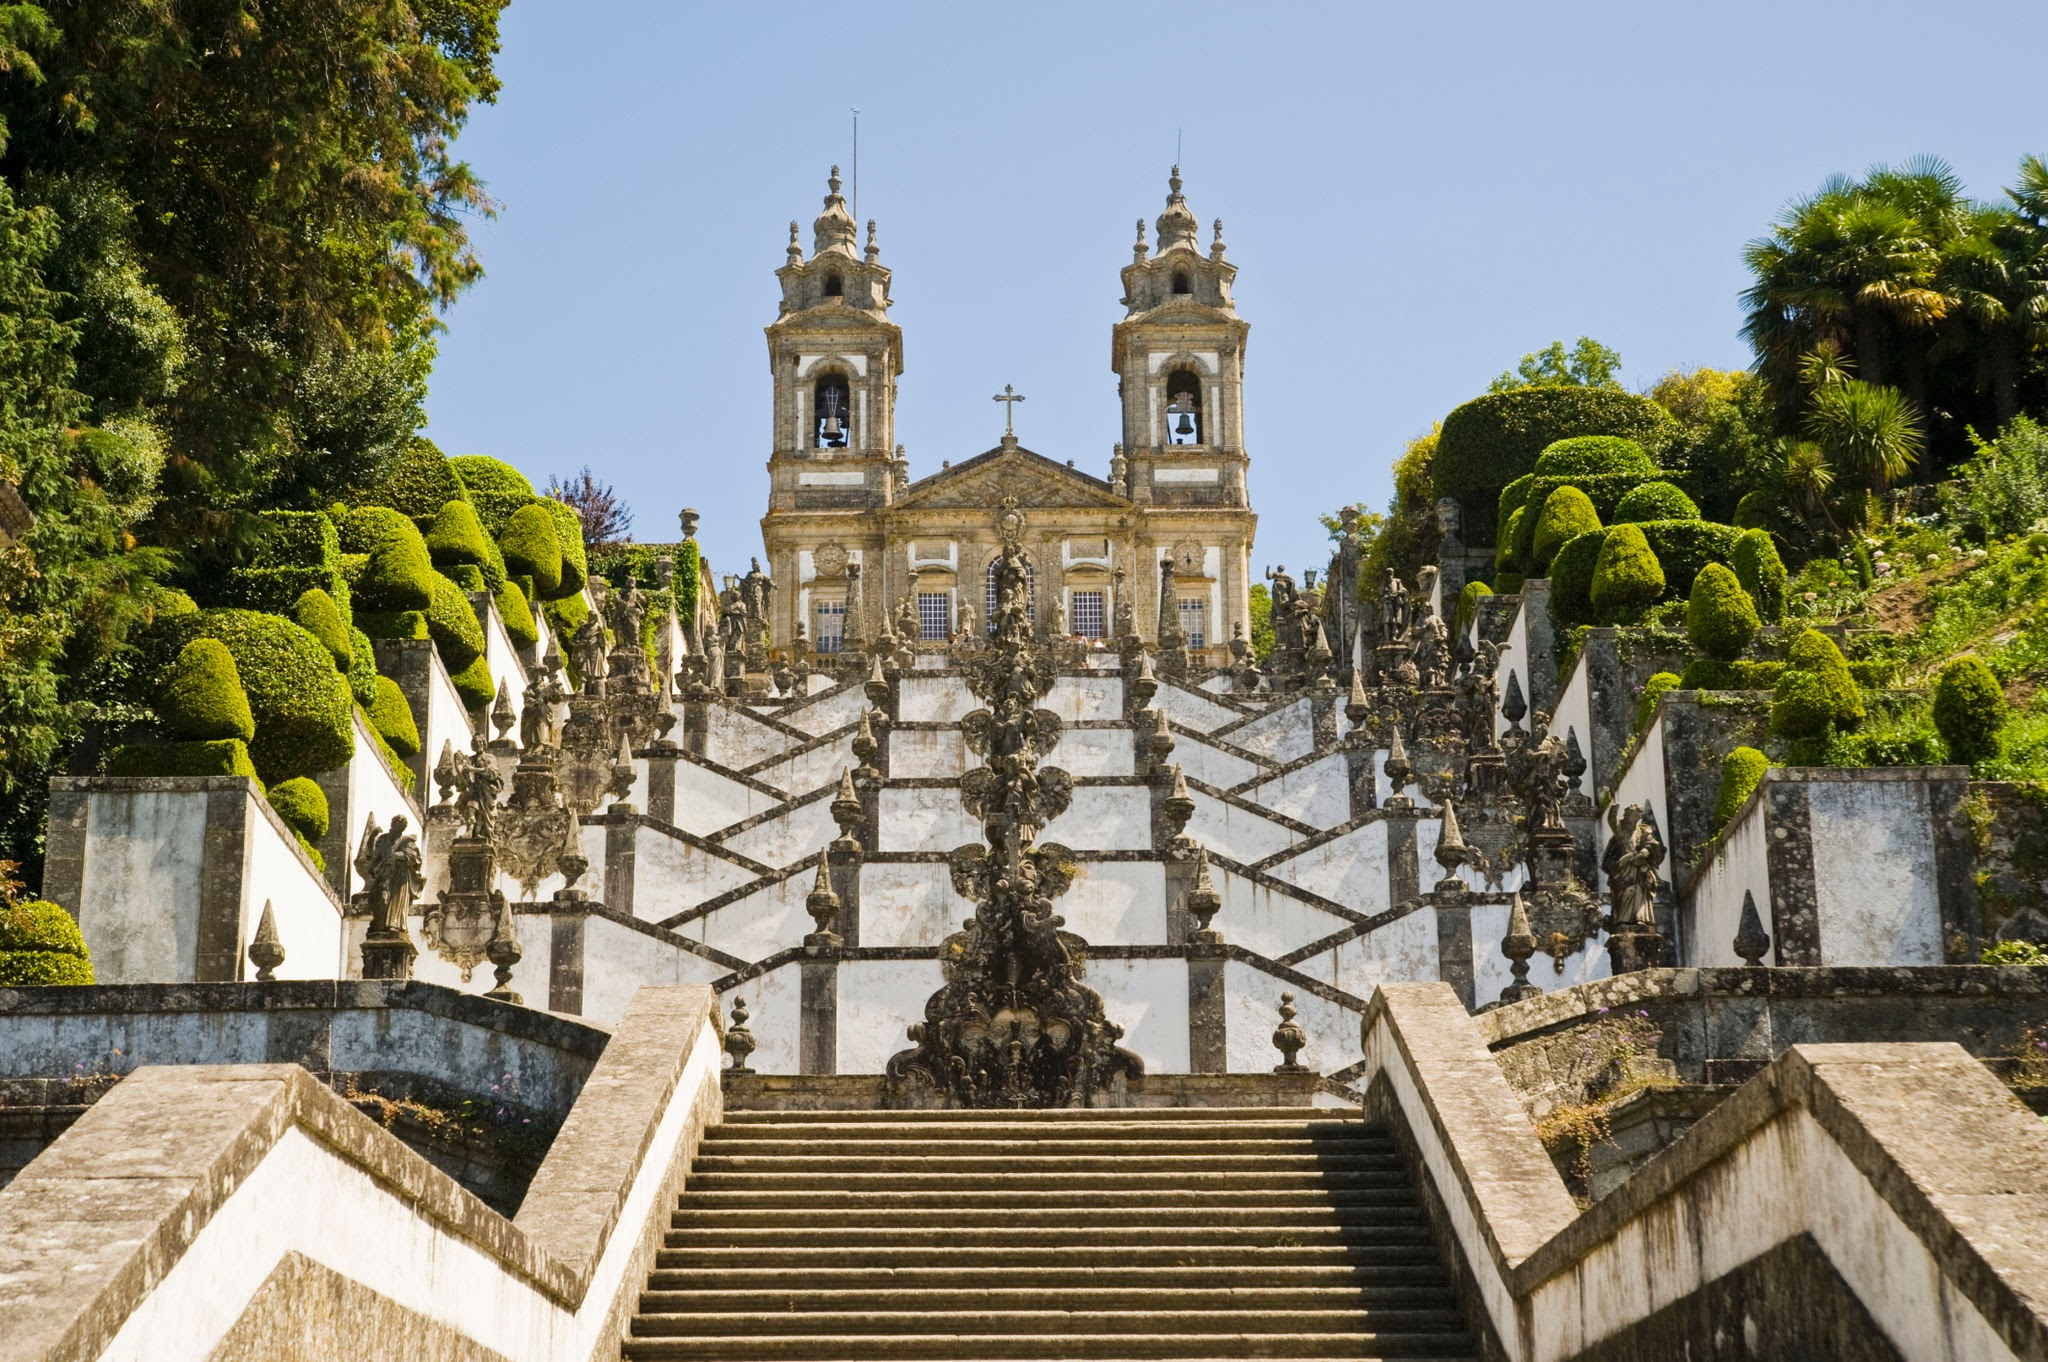
\includegraphics[width=14cm]{logoBraga.jpeg}%
\vspace{1cm}
\begin{Large}
\\
Training to share knowledge and experiences in implementing AI at schools \\
LTTA June 2022 \\
Braga, Portugal, May 31\textsuperscript{st} - June 3\textsuperscript{rd}, 2022 \\
\end{Large}
\vfill
}}}
%%%
% custom titlepage
\makeatletter
\renewcommand{\maketitle}{
\thispagestyle{empty}
\AddToShipoutPicture*{\BackgroundPic}
\ClearShipoutPicture
%
\phantom{a}
\vfill
\phantom{a}\hfill
\begin{tabular}[c]{@{}p{0.7\textwidth}@{}}
      \color{white}\headingfont\LARGE\@title\\[1em]
      \color{white}\headingfont\Large\@author\\[2em]
\end{tabular}
%
\clearpage
}
\makeatother
%%%


%%% fancy boxes
\usepackage{tcolorbox}
\usepackage{wrapfig}
%\def\namesurname{\color{xº}\headingfont\bfseries\uppercase}{\thesubsubsection}{1em}{}

\def\fullboxbegin{
\bigskip
\begin{tcolorbox}[colback=color1,colframe=color1,coltext=white,arc=0mm,boxrule=0pt]
}
\def\fullboxend{\end{tcolorbox}\medskip}
%
\def\leftboxbegin{
\begin{wrapfigure}{l}{0.5\textwidth}
\begin{tcolorbox}[colback=color1,colframe=color1,coltext=white,arc=0mm,boxrule=0pt]
}
\def\leftboxend{
\end{tcolorbox}
\end{wrapfigure}
}
%
\def\rightboxbegin{
\begin{wrapfigure}{r}{0.5\textwidth}
\begin{tcolorbox}[colback=color1,colframe=color1,coltext=white,arc=0mm,boxrule=0pt]
}
\def\rightboxend{
\end{tcolorbox}
\end{wrapfigure}
}
%
\newcounter{frames}
\def\frameboxbegin#1{
\bigskip
\refstepcounter{frames}
\begin{tcolorbox}[colback=white,colframe=color1,arc=0mm,title={\MakeUppercase{#1}}]
}
\def\frameboxend{
\end{tcolorbox}
}
%%%


\usepackage{lipsum}
\usepackage[spanish]{babel}
\setcounter{page}{0}

%%%%%%%%%%%%%%%
% Title Page
\title{}
\author{}
\date{}
%%%%%%%%%%%%%%%

\begin{document}
\maketitle

%\tableofcontents
\clearpage

\section*{Participants}
\noindent
\begin{minipage}{0.3\textwidth}
\centering
\includegraphics[width=5cm]{images/img1.jpeg}
\end{minipage}
\hfill
\begin{minipage}{0.6\textwidth}\raggedright
\color{color1}\uppercase{\textbf{Marjon Blondeel}}
\color{color2}\hspace{0.2cm}\includegraphics{flags/be.png}
\\
software/AI developer at VUB\\
{\footnotesize Researcher in AI until 2015. Now focused on developing AI applications and giving trainings on AI. During 1 year I also worked as a teacher in secondary school and I have many years of experience as a teaching assistant and lecturer in higher education. I've taught basic courses for informatics students, but also programming courses for other students such as Bio-Engineering students. }\\
\end{minipage}
\newline\newline\newline

\noindent
\begin{minipage}{0.3\textwidth}
\centering
\includegraphics[height=5cm]{images/img0.jpg}
\end{minipage}
\hfill
\begin{minipage}{0.6\textwidth}\raggedright
\color{color1}\uppercase{\textbf{Macu Caruana}}
\color{color2}\hspace{0.2cm}\includegraphics{flags/es.png}
\hspace{0.2cm}\textit{@macucaruana}
\\
Primary Teacher at Teacher\\
{\footnotesize Keen on Technology and education. I love sports, fan of Rafa Nadal. I also like photography and living as close as possible to the sea.}\\
\end{minipage}
\newline\newline\newline

\noindent
\begin{minipage}{0.3\textwidth}
\centering
\includegraphics[height=5cm]{images/img3.png}
\end{minipage}
\hfill
\begin{minipage}{0.6\textwidth}\raggedright
\color{color1}\uppercase{\textbf{Meritxell Díaz Coque}}
\color{color2}\hspace{0.2cm}\includegraphics{flags/es.png}
\\
Researcher at King Juan Carlos University\\
{\footnotesize I am a Electrical Engineer in Telecommunications and in Aerospace Engineer, currently working as a researcher in the FAIaS project. In this project, we are trying to teach Artificial Intelligence in high schools. I'm passionate about programming and artificial intelligence.}\\
\end{minipage}
\newline\newline\newline

\noindent
\begin{minipage}{0.3\textwidth}
\centering
\includegraphics[height=5cm]{images/img0.jpg}
\end{minipage}
\hfill
\begin{minipage}{0.6\textwidth}\raggedright
\color{color1}\uppercase{\textbf{Johan Loeckx}}
\color{color2}\hspace{0.2cm}\includegraphics{flags/be.png}
\hspace{0.2cm}\textit{@aibrussels}
\\
Researcher at Artificial Intelligence Lab Brussels (VUB)\\
{\footnotesize I have three passions: music, education \& AI.  have founded a Freinet school in Brussels, I have done research on using AI to educate people on music, and am currently mainly involved with lifelong learning of AI.}\\
\end{minipage}
\newline\newline\newline

\noindent
\begin{minipage}{0.3\textwidth}
\centering
\includegraphics[height=5cm]{images/img5.jpeg}
\end{minipage}
\hfill
\begin{minipage}{0.6\textwidth}\raggedright
\color{color1}\uppercase{\textbf{Gregorio Robles}}
\color{color2}\hspace{0.2cm}\includegraphics{flags/es.png}
\hspace{0.2cm}\textit{@gregoriorobles}
\\
Full Professor at Universidad Rey Juan Carlos\\
{\footnotesize I am a Full Professor at the Universidad Rey Juan Carlos, a public university in the South of Madrid.}\\
\includegraphics[height=0.35cm]{figs/internet.png}\hspace{0.1cm}{\footnotesize \color{color1}\url{https://gsyc.urjc.es/~grex/}}
\end{minipage}
\newline\newline\newline

\noindent
\begin{minipage}{0.3\textwidth}
\centering
\includegraphics[width=5cm]{images/img6.png}
\end{minipage}
\hfill
\begin{minipage}{0.6\textwidth}\raggedright
\color{color1}\uppercase{\textbf{Pablo Duo Terron}}
\color{color2}\hspace{0.2cm}\includegraphics{flags/es.png}
\hspace{0.2cm}\textit{@esparaTIC}
\\
Director and teacher  in Primary School at ministry of education and vocational training\\
{\footnotesize Doctoral student in education 
Master TIC and Educational Inspection 
Degree in primary school and physical education  
2nd best teacher of Primary School in Spain 2021
Coordinator and tutor of the Future Classroom courses of the (national institute of technology teacher training in Spain) INTEF
Tutor of the Computational Thinking and Artificial Intelligence school of the INTEF
STEM Diagnostic Test Coordinator INEE}\\
\includegraphics[height=0.35cm]{figs/internet.png}\hspace{0.1cm}{\footnotesize \color{color1}\url{educaciontic.es}}
\end{minipage}
\newline\newline\newline



\end{document}
